\section{Introduction}

Since 1980, there has been a notable divergence in performance between CPUs and DRAM.
To bridge this gap, architects introduced small, high-speed cache memories between the CPU and DRAM, establishing a memory hierarchy.
With the advent of recent multicore processors, the design of memory hierarchy has become increasingly critical. 
To address this challenge, several solutions are necessary: multi-port pipelined caches, two-level cache structure per core, and shared third-level cache on chip: Integrating a shared third-level cache directly on the chip further streamlines memory access.

The ultimate goal of the memory hierarchy is to create the illusion of a vast, speedy, and cost-effective memory system.
This allows programs to access a memory space scalable to the size of the disk, with speeds comparable to register access. 
Achieving this necessitates the establishment of a memory hierarchy comprising various technologies, costs, and sizes, each with distinct access mechanisms.
\begin{figure}[H]
    \centering
    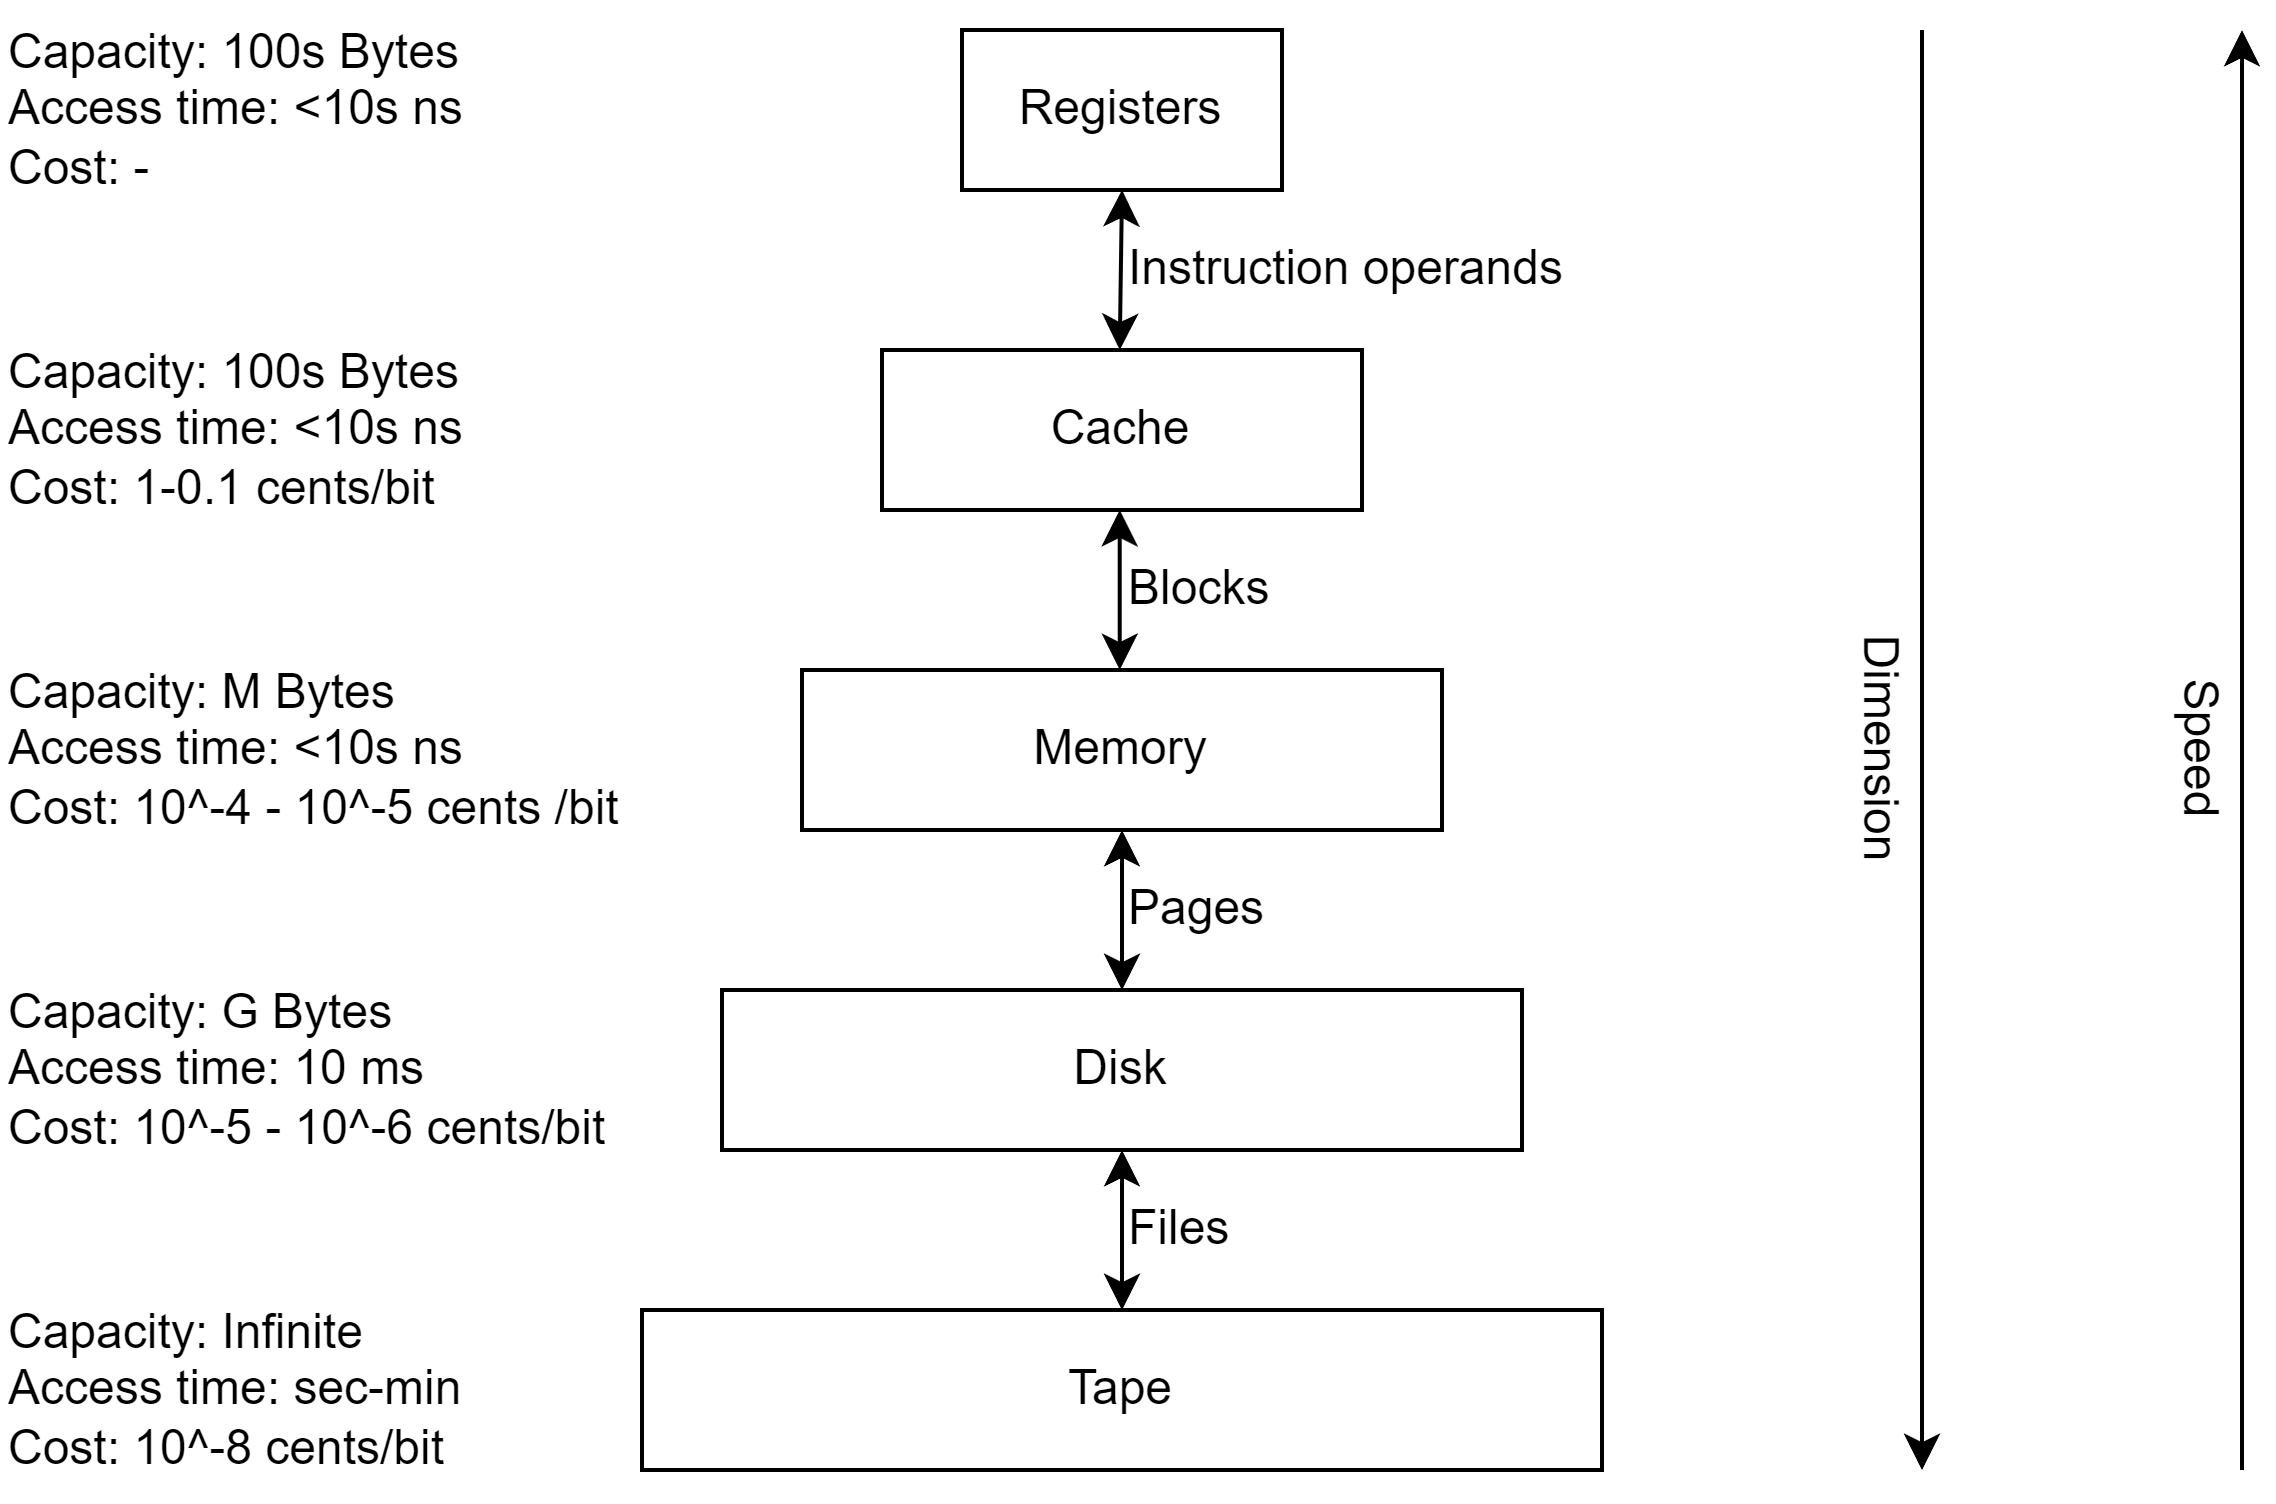
\includegraphics[width=0.7\linewidth]{images/hierarchy.png}
    \caption{Memory hierarchy}
\end{figure}